%
%       Abstract
%
\begin{abstract}
    In this report we present an implementation in C of a program which computes
    the Mandelbrot set in a parallel and distributed environment. To achieve
    this, we use the OpenMP and MPI libraries respectively. We perform 
    multiple tests to evaluate the performance of our implementation, varying
    the amount of resources used and the number of processes. All the tests
    are performed on the ORFEO cluster of the Area Science Park. Finally we
    compare the results obtained with the theoretical expectations.
\end{abstract}

\maketitle

\section{Introduction to the problem}
    The Mandelbrot set is the set of all complex numbers $c$ for
    which the sequence defined by $z_{n+1} = z_n^2 + c$ does not diverge.
    In this report we implement a C code which computes the Mandelbrot set
    point by point and then save the result as a PGM image. The computation
    of each point is independent of the others, so we can easily parallelize
    the computation and distribute it among multiple processes to speed up
    the computation. We use the OpenMP and MPI libraries to achieve this.
\subsection{Arithmetic Intesity}
    The arithmetic intensity of a program is defined as the ratio of the
    number of arithmetic operations to the number of memory operations.
    In our case we have:
    \begin{itemize}
        \item 2 mult and 1 add: \texttt{z.x*z.x+z.y*z.y}
        \item 2 mult, 1 sub and 1 add: \texttt{temp=z.x*z.x-z.y*z.y+c.x}
        \item 2 mult and 1 add: \texttt{z.y=2*z.x*z.y+c.y}
        \item 1 add: \texttt{++n}
    \end{itemize}
    for a total of 11 arithmetic operations. The memory operations are:
    \begin{itemize}
        \item 1 write: \texttt{int n = 0} 
        \item 2 writes: \texttt{Complex z = \{0,0\}}
        \item 2 reads: \texttt{z.x*z.x+z.y*z.y}
        \item 3 reads and 1 write: \texttt{temp=z.x*z.x-z.y*z.y+c.x}
        \item 3 reads and 1 write: \texttt{z.y=2*z.x*z.y+c.y}
        \item 1 write: \texttt{z.x=temp}
        \item 1 write: \texttt{++n}
    \end{itemize}
    for a total of 13 memory operations. The arithmetic intensity is then
    $$
        \frac{11 \cdot N}{ 10\cdot N + 3} 
        = \frac{11}{10+\frac{3}{N}} \xrightarrow{N \to \infty} \frac{11}{10}
        = 1.1 \text{ flops/byte}
    $$
    This value is slightly greater than 1, which means that the computation
    is compute-bound when the number of iterations is large, memory-bound
    otherwise. Notice that we did not consider the memory operations
    required to store the result of the computation nor the comparisons in
    the conditional statement. Anyway we also did not consider the effect
    of the cache, which significantly reduces the time to access the memory.


\section{Implementation}
    We begin by showing how the basic functions of the program work. We then
    show how we parallelize the computation using OpenMP and MPI. \\
    The value of a point in the Mandelbrot set is computed by iterating the
    aforementioned sequence, this is achieved with the \texttt{mandelbrot}
    function. This function is invoked for each point in the image by the
    \texttt{mandelbrot\_set} function. Finally, the result is saved as a PGM
    image by the \texttt{save\_image} function. Some important constants are
    defined with preprocessor directives:
    \begin{itemize}
        \item \texttt{WIDTH} and \texttt{HEIGHT} define the dimensions of the
            image.
        \item \texttt{MAX\_ITER} defines the maximum number of iterations
            before we consider a point to be in the Mandelbrot set.
        \item \texttt{X\_MIN}, \texttt{X\_MAX}, \texttt{Y\_MIN} and \texttt{Y\_MAX}
            define the region of the complex plane we are interested in.
    \end{itemize}
    The image array is considered a 1-dimension array allocated contiguously
    in memory with the \texttt{calloc} function. This also initialize each
    element to 0.

\subsection{Hardware}
    All the test have been performed on the ORFEO cluster of the Area Science
    Park, more specifically on the \texttt{THIN} partition. This is formed
    by $10$ nodes, each with $2$ Intel Xeon Gold 6126 processors and 768 GB of
    RAM. The nodes are interconnected with a 100 Gbit HDR Infiniband network,
    this allows a fast communication between the nodes with low latency.

\subsection{Parallel Implementation}
    To parallelize the computation of the Mandelbrot with OpenMP we have to
    make some modifications to the code. First we define the number of threads
    to be used with the environment variable \texttt{OMP\_NUM\_THREADS}.
    The part of the code we want to parallelize is the loop in the \texttt{mandelbrot\_set}
    function which iterate over all the points in the image. We add the directive
    \texttt{\#pragma omp parallel for schedule $($dynamic, OMP\_CHUNK\_SIZE$)$} before
    the loop to parallelize it. The \texttt{schedule} clause is used to specify how
    the scheduler should distribute the iterations among the threads. The \texttt{dynamic}
    option tells the scheduler to assign chunks of iterations to the threads as they
    finish their work. This is useful when the time to compute each iteration is not
    constant, as is the case with the Mandelbrot set in which few points require
    a high number of iterations to be computed. By defining the \texttt{OMP\_CHUNK\_SIZE}
    constant we can control the size of the chunks of iterations assigned to each thread.
    By default this value is set to 1. By increasing it to 4 we slightly reduce the overhead
    of the scheduler without risking load imbalance among the threads. \\

\subsection{Distributed Implementation}
    To distribute the computation of the Mandelbrot set among multiple processes
    we use the Message Passing Interface (MPI) library. Unlike OpenMP, MPI require
    a more complex setup. Here we have to explicitly define the communication
    between the processes. The main idea is to divide the image into multiple
    chunks, each of size \texttt{MPI\_CHUNK\_SIZE}, build a work queue with the
    chunks and then distribute the work among the processes. The queue structure
    is provided by the library \texttt{sys/queue.h}, each element of the queue
    is a \texttt{struct} which contains the starting point of the chunk, the
    ending point and a pointer to the next element. After having built the queue,
    the master process sends a chunk to each worker process with the function
    \texttt{MPI\_Send}. We keep track of which process is working with the
    \texttt{processes\_status} array: a value of 0 means the process is idle, a
    value of 1 means the process is working. We also keep track of the overall
    number of chunks that have been completed with the \texttt{completed\_chunks}
    variable and the number of available chunks with the \texttt{available\_chunks}
    variable. The available chunks are the ones that are not already assigned 
    to a process. If the number of available chunks is greater than 0, the master
    process assign a work chunks to itself, without using any MPI function obviously.
    As a consequence, the master process has two responsibilities: to compute
    the mandelbrot set (as any other process) and to distribute the work among
    the processes. When a worker process has finished its computation, it sends
    back the result to the master process with the function \texttt{MPI\_Send}.
    Eventually, when the work queue has been emptied, the master process sends
    a stop message to the idle processes. \\
    By dynamically assigning the chunks to the processes we aim to reduce the
    load imbalance among the processes. Basically we reproduce the same mechanism
    OpenMP adopts to distribute the iterations among the threads when the 
    \texttt{dynamic} schedule is used.

\subsection{Hybrid Implementation}
    We can combine the OpenMP and MPI libraries to achieve a hybrid implementation
    of the Mandelbrot set computation. The idea is to use MPI to distribute the
    work among the processes and then use OpenMP to parallelize the computation
    of each chunk. Recall that the implementation of both OpenMP and MPI is
    scheduling the work dynamically, so we expect a good load balance among the
    threads and the processes. The size of the chunks assigned to each MPI process
    is not trivial to determine, and a further step of optimization could be
    to adaptively change the size of the chunks depending on the resolution
    of the image and the number of processes. This is left as a future work.

\section{Scalability}
    We evaluate the performance of our implementation by assessing its scalability
    in a strong and a weak sense. For both cases we scale once the number of OMP threads
    and once the number of MPI processes. Again, for each case we compute the
    image of the Mandelbrot set with two different resolutions: $512 \times 512$
    and $4096 \times 4096$. We then compare the results with the theoretical
    expectations.

\subsection{Amdahl's Law}
    The theoretical speedup determined by Amdahl's law is given by
    $$
        S_p = \frac{T_1}{T_p} = \frac{1}{(1-P)+\frac{P}{N}}
    $$
    where $T_1$ is the time to solve the problem with one process, $T_p$ is the
    time to solve the problem with $P$ processes, $N$ is the number of processors
    and $P$ is the fraction of the program that can be parallelized.
    In our case, we will estimate the proportion of parallelizable code
    by measuring the time to solve the problem with two processors and then
    solve $P = 2 \left (1 - T_2/T_1 \right )$. We will then asses if the
    theoretical speedup is consistent with the experimental results for all
    the number of processors. \\

\subsection{Strong Scaling}
    By strong scaling we mean the ability of the program to solve a problem
    of fixed size in less time by using more computational resources. In our
    case, the problem size is the resolution of the image, while the computational
    resources are the number of threads or processes.
\subsubsection{MPI}
    We begin by showing the results of the strong scaling with MPI compared
    with the theoretical expectations according to Amdahl's law with $P = 1$.
    The benchmark has been performed using $4$ nodes of the cluster with $24$
    cores each. The MPI processes have been distributed among the nodes in
    such a way that each node has the same number of processes. This is done
    by using the \texttt{--map-by ppr:\enquote{processes per node}:node} option
    of the \texttt{mpiexec} command. The results are shown in the following
    figures.
    \begin{figure}[H]
        \centering
        \resizebox{0.45\textwidth}{!}{
        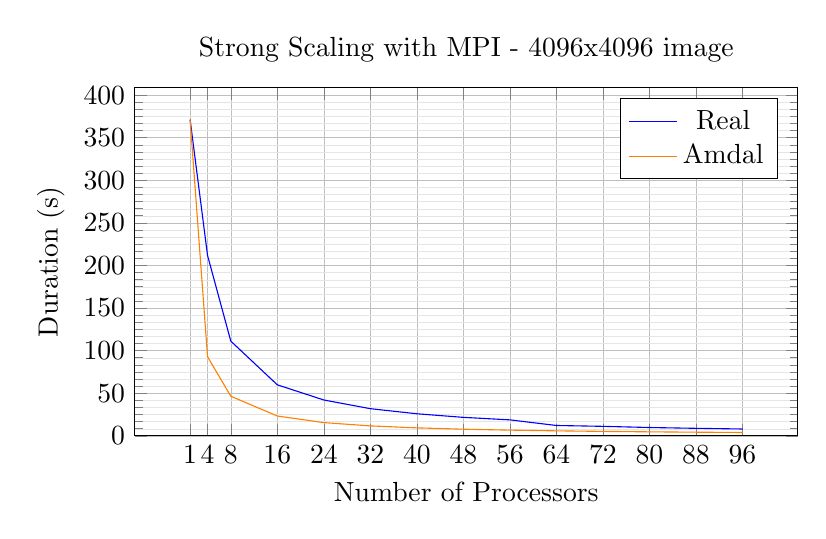
\begin{tikzpicture}
            \begin{axis}[
                title={Strong Scaling with MPI - 4096x4096 image},
                xlabel={Number of Processors},
                ylabel={Duration (s)},
                legend pos=north east,
                grid=both,
                grid style={line width=.1pt, draw=gray!20},
                major grid style={line width=.2pt,draw=gray!50},
                minor tick num=5,
                xtick={1,4,8,16,24,32,40,48,56,64,72,80,88,96},
                % xmode=log,
                % log basis x={2},
                ymin=0,
                % xmin=0,
                % xmax=100,
                ytick={0, 50, 100, 150, 200, 250, 300, 350, 400},
                width=10cm,
                height=6cm,
                % cycle list name=color list,
            ]
            
            % Blue line: Real
            \addplot[
                color=blue,
                mark=none,
                ]
                coordinates {
                (1, 371.358653)
                (4, 211.746975)
                (8, 111.103532)
                (16, 59.841779)
                (24, 42.016501)
                (32, 31.829848)
                (40, 25.848301)
                (48, 21.634139)
                (56, 18.693487)
                (64, 12.088247)
                (72, 11.09093)
                (80, 9.714115)
                (88, 8.76143)
                (96, 7.975981)
                };
                \addlegendentry{Real}
            
            % Orange line: Amdal
            \addplot[
                color=orange,
                mark=none,
                ]
                coordinates {
                (1, 371.358653)
                (4, 92.83966325)
                (8, 46.419831625)
                (16, 23.2099158125)
                (24, 15.473277208333332)
                (32, 11.60495790625)
                (40, 9.283966325)
                (48, 7.736638604166666)
                (56, 6.631404517857143)
                (64, 5.802478953125)
                (72, 5.157759069444444)
                (80, 4.6419831625)
                (88, 4.219984693181818)
                (96, 3.868319302083333)
                };
                \addlegendentry{Amdal}
            
            \end{axis}
        \end{tikzpicture}
        }
    \end{figure}
    \begin{figure}[H]
        \centering
        \resizebox{0.45\textwidth}{!}{
        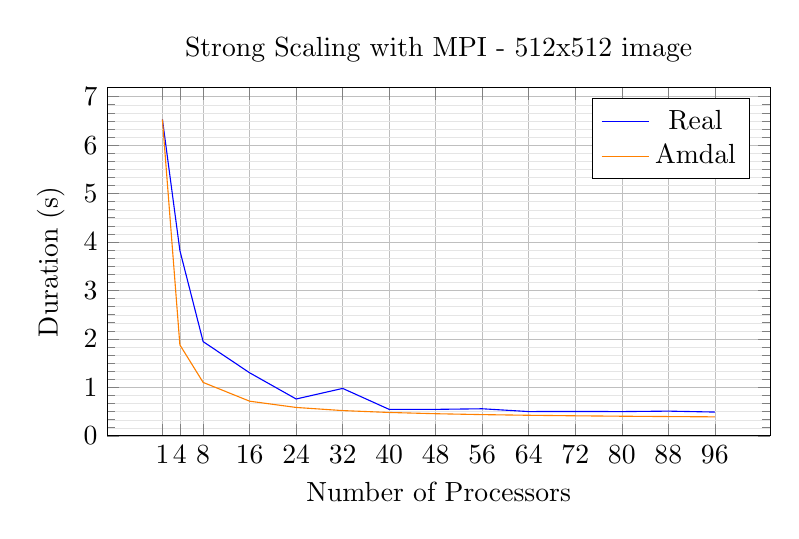
\begin{tikzpicture}
            \begin{axis}[
                title={Strong Scaling with MPI - 512x512 image},
                xlabel={Number of Processors},
                ylabel={Duration (s)},
                legend pos=north east,
                grid=both,
                grid style={line width=.1pt, draw=gray!20},
                major grid style={line width=.2pt,draw=gray!50},
                minor tick num=5,
                xtick={1,4,8,16,24,32,40,48,56,64,72,80,88,96},
                % xmode=log,
                % log basis x={2},
                ymin=0,
                % xmin=0,
                % xmax=100,
                ytick={0, 1, 2, 3, 4, 5, 6, 7},
                width=10cm,
                height=6cm,
                % cycle list name=color list,
            ]
            % real  [6.528405, 3.824648, 1.943719, 1.300054, 0.759538, 0.977942, 0.544757, 0.545445, 0.557732, 0.499887, 0.502379, 0.499451, 0.509071, 0.489834]
            % amdal  [6.528405, 1.8769164375000003, 1.1016683437500003, 0.7140442968750003, 0.5848362812500003, 0.5202322734375003, 0.48146986875000025, 0.4556282656250003, 0.4371699776785717, 0.4233262617187503, 0.4125589270833336, 0.4039450593750003, 0.3968973494318185, 0.3910242578125003]
            % Blue line: Real
            \addplot[
                color=blue,
                mark=none,
                ]
                coordinates {
                (1, 6.528405)
                (4, 3.824648)
                (8, 1.943719)
                (16, 1.300054)
                (24, 0.759538)
                (32, 0.977942)
                (40, 0.544757)
                (48, 0.545445)
                (56, 0.557732)
                (64, 0.499887)
                (72, 0.502379)
                (80, 0.499451)
                (88, 0.509071)
                (96, 0.489834)
                };
                \addlegendentry{Real}
            
            % Orange line: Amdal
            \addplot[
                color=orange,
                mark=none,
                ]
                coordinates {
                (1, 6.528405)
                (4, 1.8769164375000003)
                (8, 1.1016683437500003)
                (16, 0.7140442968750003)
                (24, 0.5848362812500003)
                (32, 0.5202322734375003)
                (40, 0.48146986875000025)
                (48, 0.4556282656250003)
                (56, 0.4371699776785717)
                (64, 0.4233262617187503)
                (72, 0.4125589270833336)
                (80, 0.4039450593750003)
                (88, 0.3968973494318185)
                (96, 0.3910242578125003)
                };
                \addlegendentry{Amdal}
            
            \end{axis}
        \end{tikzpicture}
        }
    \end{figure}
    As we can see, the experimental results do not match the lower bound 
    given by Amdahl's law. This is due to the fact that the assumption
    that all the program is parallelizable $(P=1)$ is not true.
    In fact, estimating the fraction of parallelizable code with the
    formula $P = 2 \left (1 - T_2/T_1 \right )$ we obtain $P_{512} = 0.83$
    and $P_{4096} = 0.86$.\\
    Considering the estimated $P_{4096}$, we can compute the theoretical
    speedup for the $4096 \times 4096$ image and again compare it with
    the experimental results.
    \begin{figure}[H]
        \centering
        \resizebox{0.45\textwidth}{!}{
        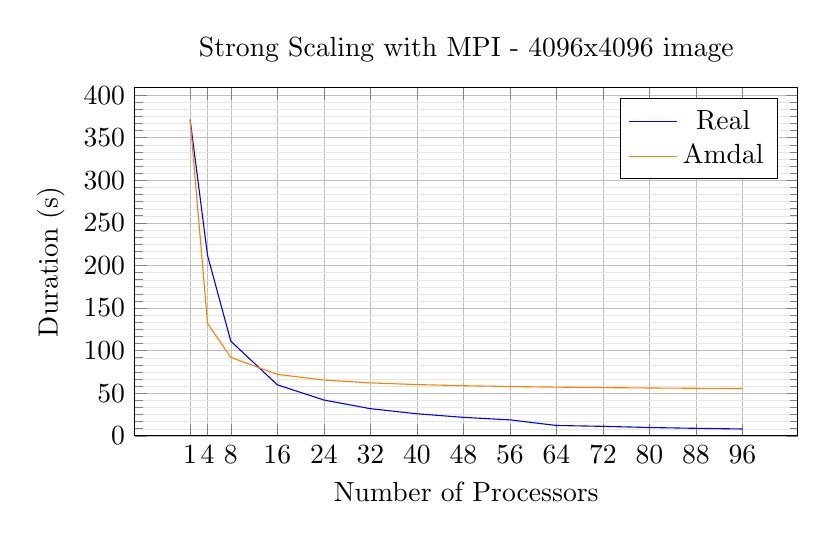
\begin{tikzpicture}
            \begin{axis}[
                title={Strong Scaling with MPI - 4096x4096 image},
                xlabel={Number of Processors},
                ylabel={Duration (s)},
                legend pos=north east,
                grid=both,
                grid style={line width=.1pt, draw=gray!20},
                major grid style={line width=.2pt,draw=gray!50},
                minor tick num=5,
                xtick={1,4,8,16,24,32,40,48,56,64,72,80,88,96},
                % xmode=log,
                % log basis x={2},
                ymin=0,
                % xmin=0,
                % xmax=100,
                ytick={0, 50, 100, 150, 200, 250, 300, 350, 400},
                width=10cm,
                height=6cm,
                % cycle list name=color list,
            ]
            
            % Blue line: Real
            \addplot[
                color=blue,
                mark=none,
                ]
                coordinates {
                (1, 371.358653)
                (4, 211.746975)
                (8, 111.103532)
                (16, 59.841779)
                (24, 42.016501)
                (32, 31.829848)
                (40, 25.848301)
                (48, 21.634139)
                (56, 18.693487)
                (64, 12.088247)
                (72, 11.09093)
                (80, 9.714115)
                (88, 8.76143)
                (96, 7.975981)
                };
                \addlegendentry{Real}
            
            % Orange line: Amdal
            % amdal: [371.358653, 131.941136, 92.03821649999999, 72.08675674999998, 65.43627016666665, 62.11102687499998, 60.115880899999986, 58.78578358333332, 57.835714071428555, 57.12316193749999, 56.56895472222221, 56.12558894999999, 55.76283513636363, 55.46054029166665]
            \addplot[
                color=orange,
                mark=none,
                ]
                coordinates {
                (1, 371.358653)
                (4, 131.941136)
                (8, 92.03821649999999)
                (16, 72.08675674999998)
                (24, 65.43627016666665)
                (32, 62.11102687499998)
                (40, 60.115880899999986)
                (48, 58.78578358333332)
                (56, 57.835714071428555)
                (64, 57.12316193749999)
                (72, 56.56895472222221)
                (80, 56.12558894999999)
                (88, 55.76283513636363)
                (96, 55.46054029166665)
                };
                \addlegendentry{Amdal}
            \end{axis}
        \end{tikzpicture}
        }
    \end{figure}
    This time we observe a different behavior. In the first part of the
    curve the experimental results lies above the theoretical expectations,
    while in the second part the experimental results lies below. This
    discrepancy can be explained by the fact that the Amdahl's law assume
    that the parameter $P$ is constant and independent from $N$.
    Remebering that the estimate has been made with the first two instancies,
    it is possible that in these first two cases the load imbalance was
    greater than in the latter ones. This would explain why the experimental
    results are above the theoretical expectations in the first part of the
    curve and below in the second part. However, the average computation times
    per process, shown in the table below, contradict this hypothesis.
    \begin{table}[H]
        \centering
        \begin{tabular}{|c|c|c|c|c|}
        \hline
        \textbf{Process} & 0 & 1 & 2 & 3 \\ \hline
        \textbf{Time} & 211.745397 & 211.746975 & 211.745469 & 211.744659 \\ \hline
        \end{tabular}
        \caption{Average computation time per process ($N=4$)}
        \label{table:transposed_values}
    \end{table}
    The case of the $512 \times 512$ image is analogous. \\
    Another possible explanation could rely in the overhead caused by the 
    initial serial part of the program. This value is constant and
    independent from the number of processes, so it is more significant
    when the number of processes is small.

\subsubsection{OpenMP}
    We now show the results of the strong scaling with OpenMP compared
    with the theoretical expectations according to Amdahl's law with $P = 1$.
    \begin{figure}[H]
        \centering
        \resizebox{0.45\textwidth}{!}{
        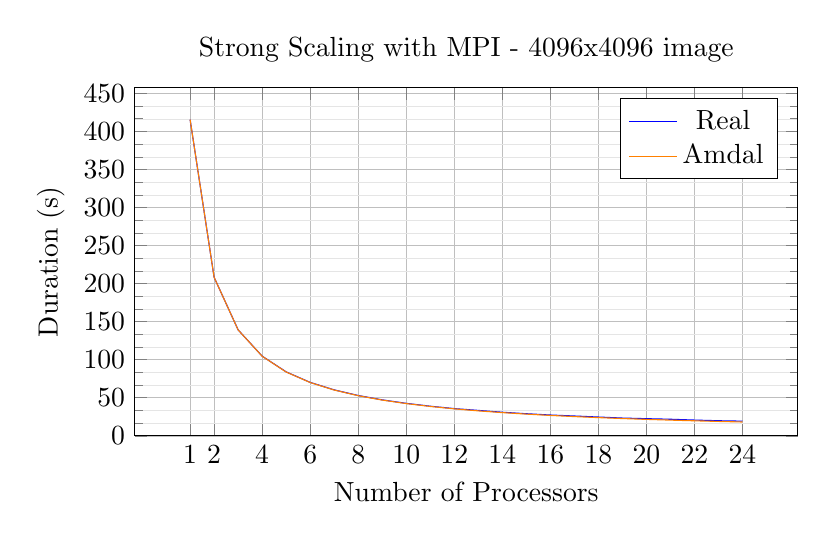
\begin{tikzpicture}
            \begin{axis}[
                title={Strong Scaling with MPI - 4096x4096 image},
                xlabel={Number of Processors},
                ylabel={Duration (s)},
                legend pos=north east,
                grid=both,
                grid style={line width=.1pt, draw=gray!20},
                major grid style={line width=.2pt,draw=gray!50},
                minor tick num=2,
                xtick={1,2,4,6,8,10,12,14,16,18,20,22,24},
                % xmode=log,
                % log basis x={2},
                ymin=0,
                % xmin=0,
                % xmax=100,
                ytick={0, 50, 100, 150, 200, 250, 300, 350, 400, 450},
                width=10cm,
                height=6cm,
                % cycle list name=color list,
            ]

            % x = [1, 2, 3, ..., 23, 24]
            % real = [415.661696, 208.247553, 139.165655, 104.656798, 83.975518, 70.16855, 60.33325, 52.92974, 47.198111, 42.618235, 38.863273, 35.710124, 33.33666762346096, 30.927101173999425, 28.976889257945583, 27.276021543253105, 25.985570873724576, 24.62994502459599, 23.28144208948935, 22.47376659569014, 21.729953256477426, 20.643902601709605, 19.759922201114204, 19.208314956723797]
            % amdal = [415.661696, 208.24755299999998, 139.10950533333332, 104.54048149999998, 83.79906719999998, 69.97145766666665, 60.09459371428571, 52.686945749999985, 46.92544177777776, 42.316238599999984, 38.54507236363634, 35.40243383333332, 32.743278153846134, 30.464001857142843, 28.488629066666654, 26.760177874999982, 25.235073882352925, 23.87942588888887, 22.66647768421051, 21.574824299999985, 20.58713790476189, 19.689241181818165, 18.86942243478259, 18.11792191666665]
            
            % Blue line: Real
            \addplot[
                color=blue,
                mark=none,
                ]
                coordinates {
                (1, 415.661696)
                (2, 208.247553)
                (3, 139.165655)
                (4, 104.656798)
                (5, 83.975518)
                (6, 70.16855)
                (7, 60.33325)
                (8, 52.92974)
                (9, 47.198111)
                (10, 42.618235)
                (11, 38.863273)
                (12, 35.710124)
                (13, 33.33666762346096)
                (14, 30.927101173999425)
                (15, 28.976889257945583)
                (16, 27.276021543253105)
                (17, 25.985570873724576)
                (18, 24.62994502459599)
                (19, 23.28144208948935)
                (20, 22.47376659569014)
                (21, 21.729953256477426)
                (22, 20.643902601709605)
                (23, 19.759922201114204)
                (24, 19.208314956723797)
                };
                \addlegendentry{Real}
            
            % Orange line: Amdal
            \addplot[
                color=orange,
                mark=none,
                ]
                coordinates {
                (1, 415.661696)
                (2, 208.24755299999998)
                (3, 139.10950533333332)
                (4, 104.54048149999998)
                (5, 83.79906719999998)
                (6, 69.97145766666665)
                (7, 60.09459371428571)
                (8, 52.686945749999985)
                (9, 46.92544177777776)
                (10, 42.316238599999984)
                (11, 38.54507236363634)
                (12, 35.40243383333332)
                (13, 32.743278153846134)
                (14, 30.464001857142843)
                (15, 28.488629066666654)
                (16, 26.760177874999982)
                (17, 25.235073882352925)
                (18, 23.87942588888887)
                (19, 22.66647768421051)
                (20, 21.574824299999985)
                (21, 20.58713790476189)
                (22, 19.689241181818165)
                (23, 18.86942243478259)
                (24, 18.11792191666665)
                };
                \addlegendentry{Amdal}
            \end{axis}
        \end{tikzpicture}
        }
    \end{figure}
    \begin{figure}[H]
        \centering
        \resizebox{0.45\textwidth}{!}{
        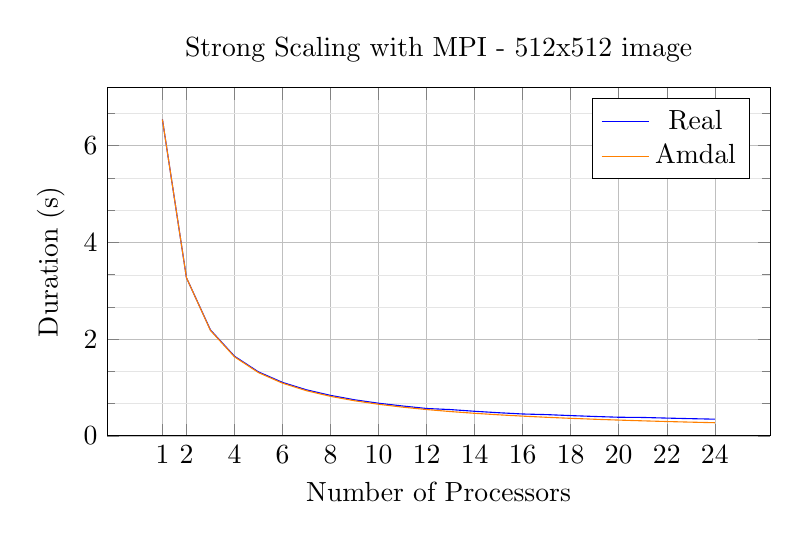
\begin{tikzpicture}
            \begin{axis}[
                title={Strong Scaling with MPI - 512x512 image},
                xlabel={Number of Processors},
                ylabel={Duration (s)},
                legend pos=north east,
                grid=both,
                grid style={line width=.1pt, draw=gray!20},
                major grid style={line width=.2pt,draw=gray!50},
                minor tick num=2,
                xtick={1,2,4,6,8,10,12,14,16,18,20,22,24},
                % xmode=log,
                % log basis x={2},
                ymin=0,
                % xmin=0,
                % xmax=100,
                % ytick={0, 50, 100, 150, 200, 250, 300, 350, 400, 450},
                width=10cm,
                height=6cm,
                % cycle list name=color list,
            ]

            % x = [1, 2, 3, ..., 23, 24]
            % real = [6.542253, 3.270055, 2.189338, 1.646339, 1.321695, 1.104557, 0.950666, 0.835814, 0.744772, 0.673606, 0.616551, 0.564914, 0.5420327788647095, 0.507226722269573, 0.47713781646738723, 0.45110666084923023, 0.438131546398441, 0.4178534199562278, 0.3998797734655113, 0.3837668738624881, 0.3793089123223544, 0.366300617912716, 0.35442535450045887, 0.34385476324907194]
            % amdal = [6.542253, 3.2700550000000006, 2.179322333333334, 1.6339560000000009, 1.306736200000001, 1.0885896666666677, 0.9327707142857153, 0.815906500000001, 0.7250121111111122, 0.652296600000001, 0.592802090909092, 0.5432233333333344, 0.501272076923078, 0.4653138571428583, 0.4341500666666678, 0.4068817500000011, 0.38282147058823635, 0.36143455555555665, 0.3422988947368432, 0.3250768000000011, 0.30949490476190583, 0.2953295454545466, 0.2823959565217402, 0.2705401666666678]
            
            % Blue line: Real
            \addplot[
                color=blue,
                mark=none,
                ]
                coordinates {
                (1, 6.542253)
                (2, 3.270055)
                (3, 2.189338)
                (4, 1.646339)
                (5, 1.321695)
                (6, 1.104557)
                (7, 0.950666)
                (8, 0.835814)
                (9, 0.744772)
                (10, 0.673606)
                (11, 0.616551)
                (12, 0.564914)
                (13, 0.5420327788647095)
                (14, 0.507226722269573)
                (15, 0.47713781646738723)
                (16, 0.45110666084923023)
                (17, 0.438131546398441)
                (18, 0.4178534199562278)
                (19, 0.3998797734655113)
                (20, 0.3837668738624881)
                (21, 0.3793089123223544)
                (22, 0.366300617912716)
                (23, 0.35442535450045887)
                (24, 0.34385476324907194)
                };
                \addlegendentry{Real}
            
            % Orange line: Amdal
            \addplot[
                color=orange,
                mark=none,
                ]
                coordinates {
                (1, 6.542253)
                (2, 3.2700550000000006)
                (3, 2.179322333333334)
                (4, 1.6339560000000009)
                (5, 1.306736200000001)
                (6, 1.0885896666666677)
                (7, 0.9327707142857153)
                (8, 0.815906500000001)
                (9, 0.7250121111111122)
                (10, 0.652296600000001)
                (11, 0.592802090909092)
                (12, 0.5432233333333344)
                (13, 0.501272076923078)
                (14, 0.4653138571428583)
                (15, 0.4341500666666678)
                (16, 0.4068817500000011)
                (17, 0.38282147058823635)
                (18, 0.36143455555555665)
                (19, 0.3422988947368432)
                (20, 0.3250768000000011)
                (21, 0.30949490476190583)
                (22, 0.2953295454545466)
                (23, 0.2823959565217402)
                (24, 0.2705401666666678)
                };
                \addlegendentry{Amdal}
            \end{axis}
        \end{tikzpicture}
        }
    \end{figure}
    This time the experimental results are consistent with the theoretical
    expectations. The estimated $P$ is this time equal to $1$ in both cases.
    After the $12$-th core, we can observe a slight increase in the
    computation time, likely due to the fact that we are now using the cpu
    of the second socket and this cause a slight increase in the latency of
    the communication between the two sockets.
    Despite the slight discrepancy in the second part, the OpenMP implementation
    scales significantly better than the MPI one. This is due to the fact that
    the overhead caused by the MPI communication and the initial setup is
    lower and almost absent.

\subsection{Weak Scaling}
    By weak scaling we mean the ability of the program to solve a problem
    in the same amount of time by using more computational resources and
    a proportionally larger problem size. The resolution of the image is
    proportionally increased with the number of threads or processes, the
    height and the width of the image are multiplied by the square root
    of the increment of computational resources.
    \begin{align*}
        W_{t+1} &= W_t \cdot \sqrt{\frac{N_{t+1}}{N_{t}}} \\
        H_{t+1} &= H_t \cdot \sqrt{\frac{N_{t+1}}{N_{t}}} \\
        \text{size}_{t+1} &= W_{t+1} \cdot W_{t+1} = W_{t} \cdot H_{t} \cdot \frac{N_{t+1}}{N_{t}}
    \end{align*}

\subsubsection{MPI}
    With the same setup as before, we show the results of the weak scaling
    with MPI. The results are shown in the following figures.

\subsubsection{OpenMP}
    We now show the results of the weak scaling with OpenMP. The results
    are shown in the following figures.
    \begin{figure}[H]
        \centering
        \resizebox{0.45\textwidth}{!}{
        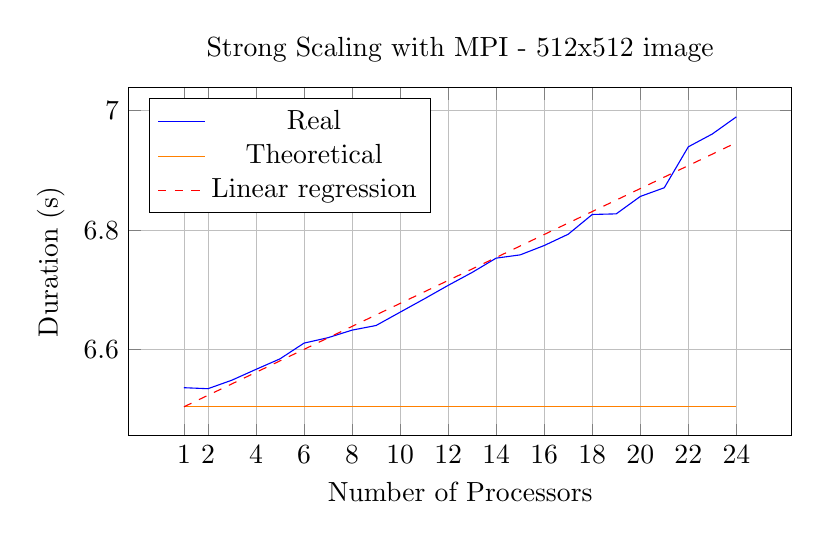
\begin{tikzpicture}
            \begin{axis}[
                title={Strong Scaling with MPI - 512x512 image},
                xlabel={Number of Processors},
                ylabel={Duration (s)},
                legend pos=north west,
                grid=both,
                grid style={line width=.1pt, draw=gray!20},
                major grid style={line width=.2pt,draw=gray!50},
                % minor tick num=2,
                xtick={1,2,4,6,8,10,12,14,16,18,20,22,24},
                % xmode=log,
                % log basis x={2},
                % ymin=6,
                % xmin=0,
                % xmax=100,
                % ytick={0, 50, 100, 150, 200, 250, 300, 350, 400, 450},
                width=10cm,
                height=6cm,
                % cycle list name=color list,
            ]

            % x = [1, 2, 3, ..., 23, 24]
            % real = [6.535942, 6.534258, 6.548605, 6.566685, 6.584302, 6.610648, 6.619744, 6.632408, 6.640174, 6.662464, 6.684632, 6.707382, 6.729084, 6.753055, 6.758507, 6.77418, 6.793104, 6.826184, 6.827232, 6.856378, 6.871, 6.939576, 6.961086, 6.989746]
            % theory = [6.535942, 6.535942, ..., 6.535942 ]
            % linreg = [6.50395693 6.52320116 6.5424454  6.56168964 6.58093388 6.60017812 6.61942236 6.63866659 6.65791083 6.67715507 6.69639931 6.71564355 6.73488779 6.75413202 6.77337626 6.7926205  6.81186474 6.83110898 6.85035322 6.86959745 6.88884169 6.90808593 6.92733017 6.94657441]
            
            % Blue line: Real
            \addplot[
                color=blue,
                mark=none,
                ]
                coordinates {
                (1, 6.535942)
                (2, 6.534258)
                (3, 6.548605)
                (4, 6.566685)
                (5, 6.584302)
                (6, 6.610648)
                (7, 6.619744)
                (8, 6.632408)
                (9, 6.640174)
                (10, 6.662464)
                (11, 6.684632)
                (12, 6.707382)
                (13, 6.729084)
                (14, 6.753055)
                (15, 6.758507)
                (16, 6.77418)
                (17, 6.793104)
                (18, 6.826184)
                (19, 6.827232)
                (20, 6.856378)
                (21, 6.871)
                (22, 6.939576)
                (23, 6.961086)
                (24, 6.989746)
                };
                \addlegendentry{Real}
            
            % Orange line: theory
            \addplot[
                color=orange,
                mark=none,
                ]
                coordinates {
                (1, 6.50395693)
                (2, 6.50395693)
                (3, 6.50395693)
                (4, 6.50395693)
                (5, 6.50395693)
                (6, 6.50395693)
                (7, 6.50395693)
                (8, 6.50395693)
                (9, 6.50395693)
                (10, 6.50395693)
                (11, 6.50395693)
                (12, 6.50395693)
                (13, 6.50395693)
                (14, 6.50395693)
                (15, 6.50395693)
                (16, 6.50395693)
                (17, 6.50395693)
                (18, 6.50395693)
                (19, 6.50395693)
                (20, 6.50395693)
                (21, 6.50395693)
                (22, 6.50395693)
                (23, 6.50395693)
                (24, 6.50395693)
                };
                \addlegendentry{Theoretical}

            % dashed red line: Linear regression
            \addplot[
                color=red,
                mark=none,
                dashed
                ]
                coordinates {
                (1, 6.50395693)
                (2, 6.52320116)
                (3, 6.5424454)
                (4, 6.56168964)
                (5, 6.58093388)
                (6, 6.60017812)
                (7, 6.61942236)
                (8, 6.63866659)
                (9, 6.65791083)
                (10, 6.67715507)
                (11, 6.69639931)
                (12, 6.71564355)
                (13, 6.73488779)
                (14, 6.75413202)
                (15, 6.77337626)
                (16, 6.7926205)
                (17, 6.81186474)
                (18, 6.83110898)
                (19, 6.85035322)
                (20, 6.86959745)
                (21, 6.88884169)
                (22, 6.90808593)
                (23, 6.92733017)
                (24, 6.94657441)
                };
                \addlegendentry{Linear regression}
            \end{axis}
        \end{tikzpicture}
        }
    \end{figure}



\section{Conclusions}
    In this work we have implemented the computation of the Mandelbrot set
    with OpenMP and MPI and we have then evaluated its performance by
    assessing its scalability in a both a strong and a weak sense. 
    When working with a single node the OpenMP implementation obviously
    outperforms the MPI one. This is due to the fact that the overhead
    caused by the MPI communication and the initial setup is absent. 
    Nonetheless, the MPI implementation allows to distribute the computation
    among multiple nodes, allowing to solve problems of larger size.
    To get the best of both worlds, we have implemented a hybrid
    version of the program, which combines the two approaches. The perfect
    setup would be to use the MPI library to distribute the work among the
    nodes and then use the OpenMP library to parallelize the computation
    on each of them.

